\documentclass[11pt,compress,t,notes=noshow, xcolor=table]{beamer}
\input{../../style/preamble_new}
\input{../../latex-math/basic-math.tex}
\input{../../latex-math/basic-ml.tex}

\title{Deep Learning for NLP}

\definecolor{texblue}{rgb}{0, 0, 1}
\def\myblue#1{\textcolor{texblue}{#1}}
\long\def\devour#1{}

\begin{document}

%\devour{

\titlemeta{
Training LLMs
}{
Scaling laws
}{
figure/losscompute.png
}{
\item Understand scaling laws
}

% ------------------------------------------------------------------------------

% ------------------------------------------------------------------------------

\begin{vbframe}{From Compute Budget to Model Design}

Training compute is approximately

\[
C \approx 6PD,
\]

where $P$ is the number of parameters and $D$ the number of training tokens.

For a fixed compute budget $C$,

\[
PD \approx \text{constant}.
\]

We can therefore spend our compute on

\begin{itemize}
    \item a \textbf{larger model} trained on fewer tokens, or
    \item a \textbf{smaller model} trained on more tokens.
\end{itemize}

\begin{center}
\textbf{Which choice gives the best model?}
\end{center}

Scaling laws help us answer this question.

\end{vbframe}
% ------------------------------------------------------------------------------

\begin{vbframe}{What Are Scaling Laws?}

\citebutton{Kaplan et al., 2020}
{https://arxiv.org/abs/2001.08361}

Language-model loss changes \textbf{predictably with scale}.

Key scaling variables are

\begin{itemize}
    \item model size $P$,
    \item training data $D$,
    \item training compute $C$.
\end{itemize}

Over large ranges, loss approximately follows power laws, e.g.,

\[
L(D) \propto D^{-\alpha}.
\]

Increasing only one factor eventually gives
\textbf{diminishing returns}.

\end{vbframe}

% ------------------------------------------------------------------------------

\begin{vbframe}{Why Were Scaling Laws Important?}

The results of Kaplan et al. were influential because they suggested that
progress from scaling was remarkably \textbf{predictable}.

\begin{itemize}
    \item Larger models and more data reliably reduced loss.
    \item Trends observed at small scale could be extrapolated
          to much larger training runs.
    \item Model \textbf{scale} mattered more than many details of
          model shape, such as depth vs.\ width.
    \item Larger models were more sample-efficient:
          they achieved a given loss with fewer training examples.
\end{itemize}

\begin{center}
\textbf{Scaling became a quantitative tool for planning LLM training.}
\end{center}

\citebutton{Kaplan et al., 2020}
{https://arxiv.org/abs/2001.08361}

\end{vbframe}

% ------------------------------------------------------------------------------

\begin{vbframe}{What Does a Power Law Look Like?}

\begin{figure}
    \centering
    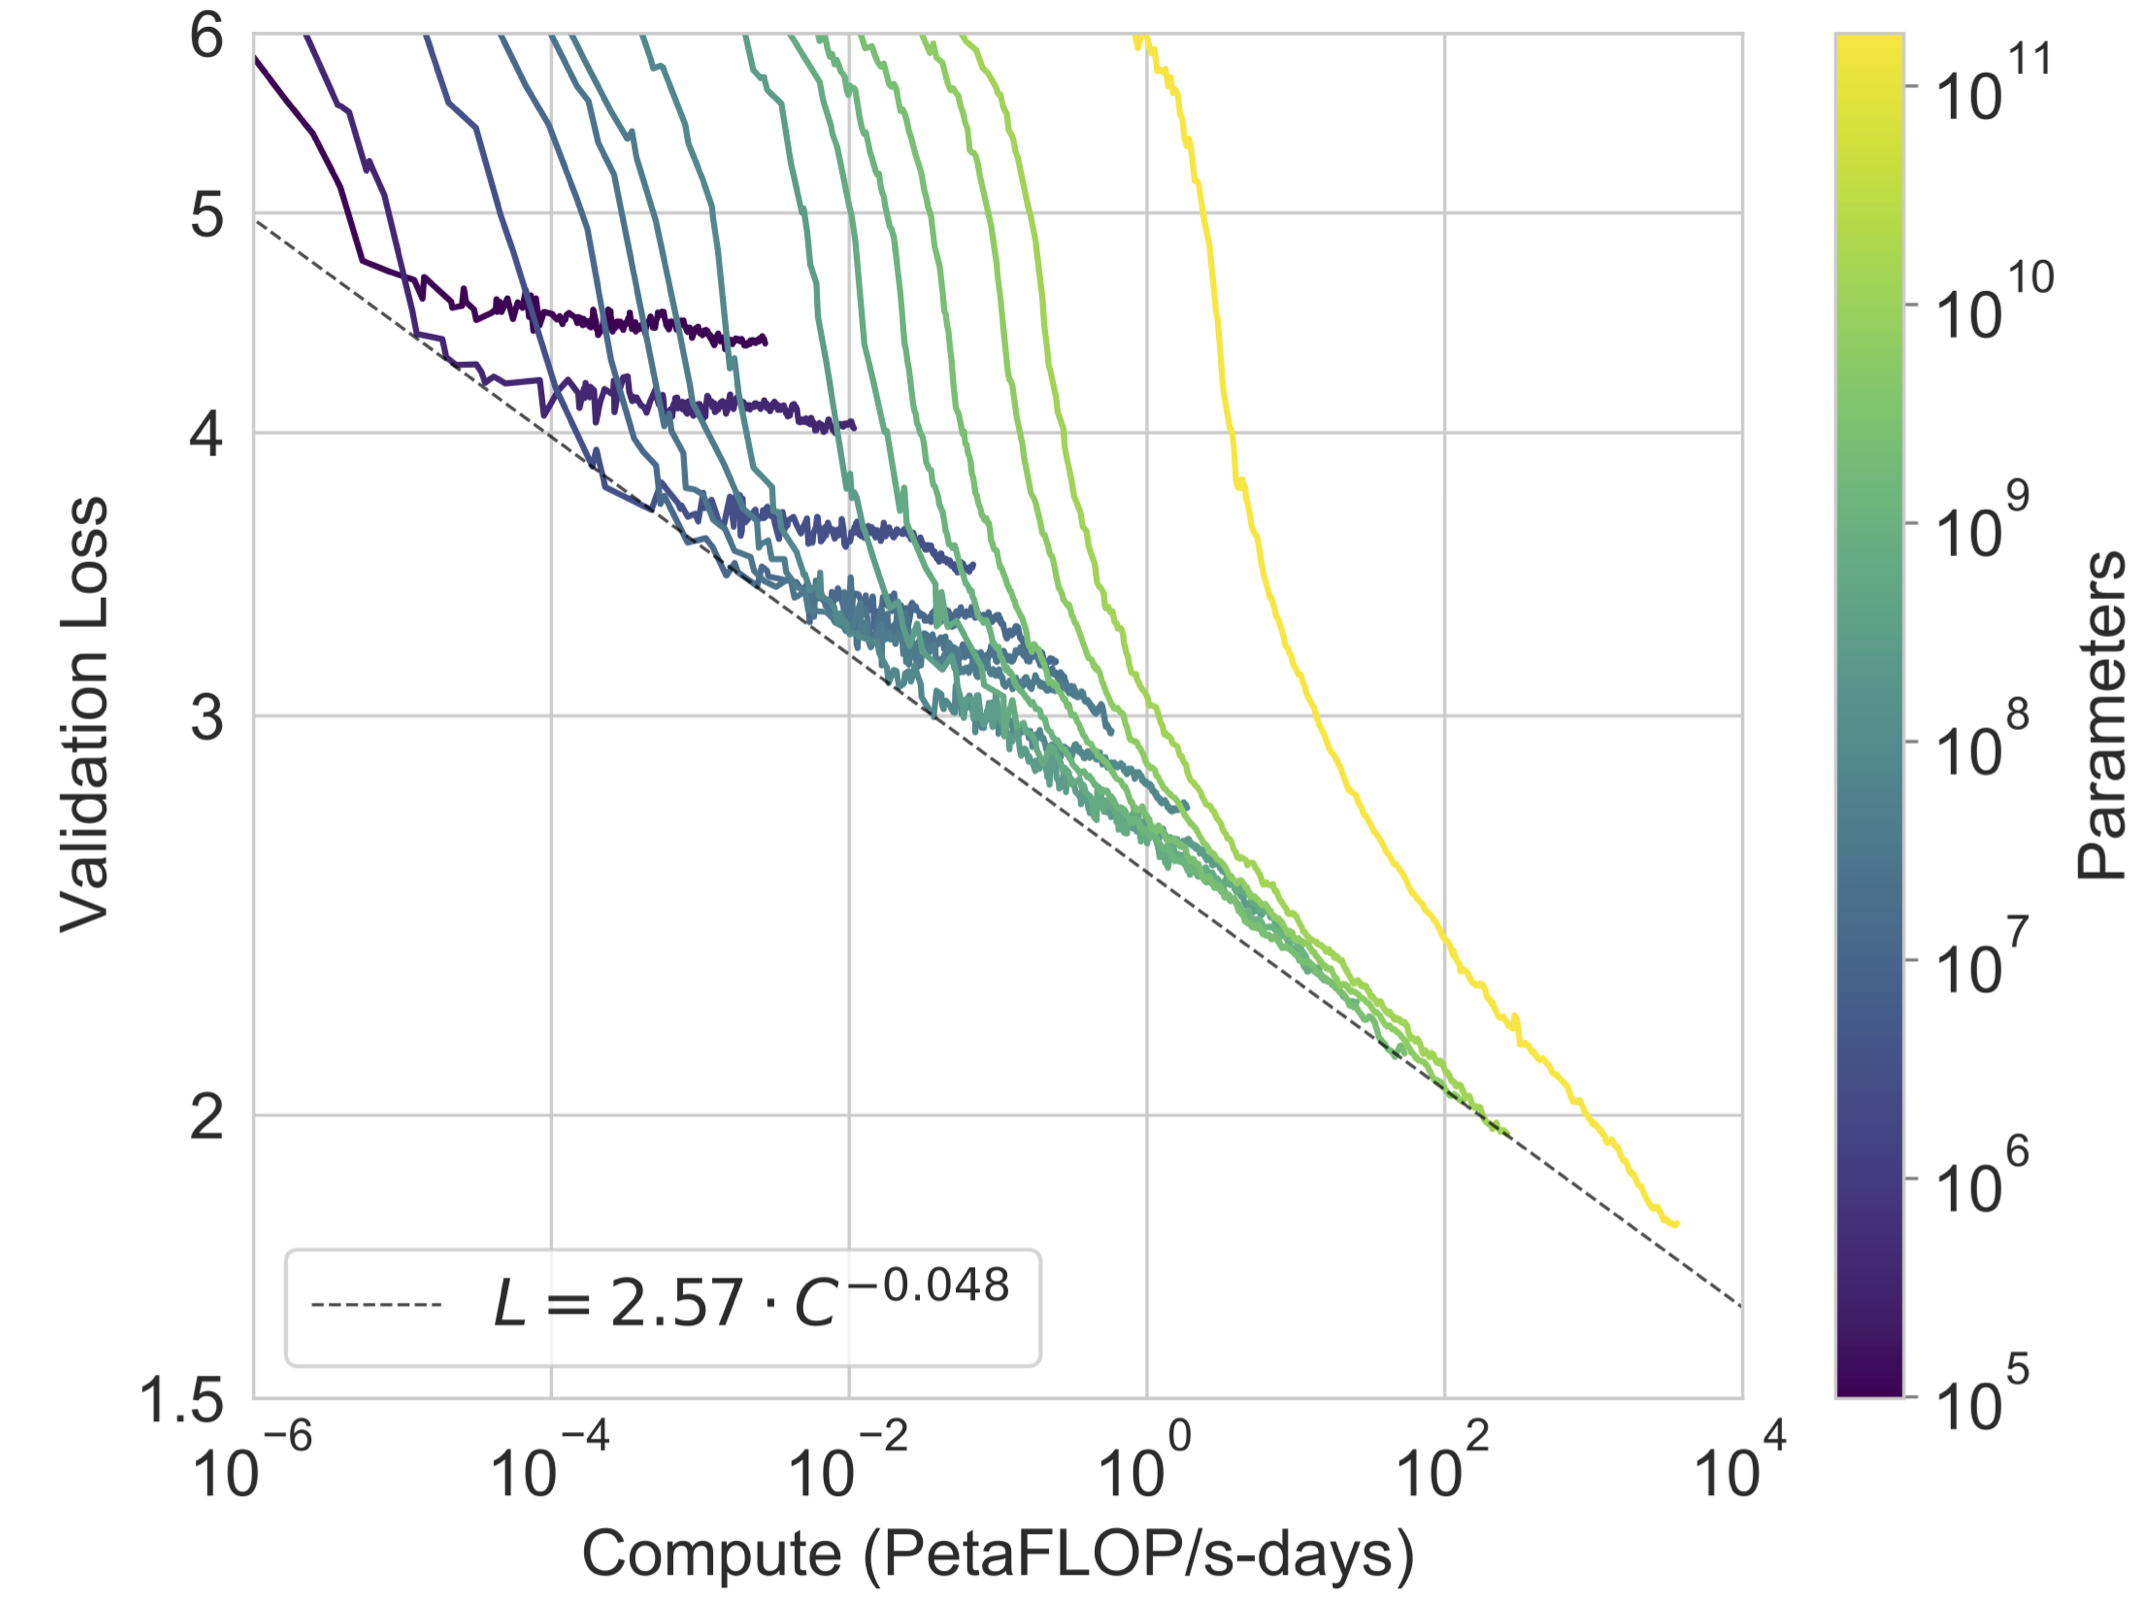
\includegraphics[width=7.5cm]{figure/losscompute.png}
\end{figure}

Validation loss decreases smoothly as training compute increases.

The approximately straight trend on log--log axes indicates
a \textbf{power law}. \citebutton{Brown et al., 2020}
{https://arxiv.org/abs/2005.14165}

\end{vbframe}

% ------------------------------------------------------------------------------

\begin{vbframe}{Scaling One Thing Is Not Enough}

\begin{figure}
    \centering
    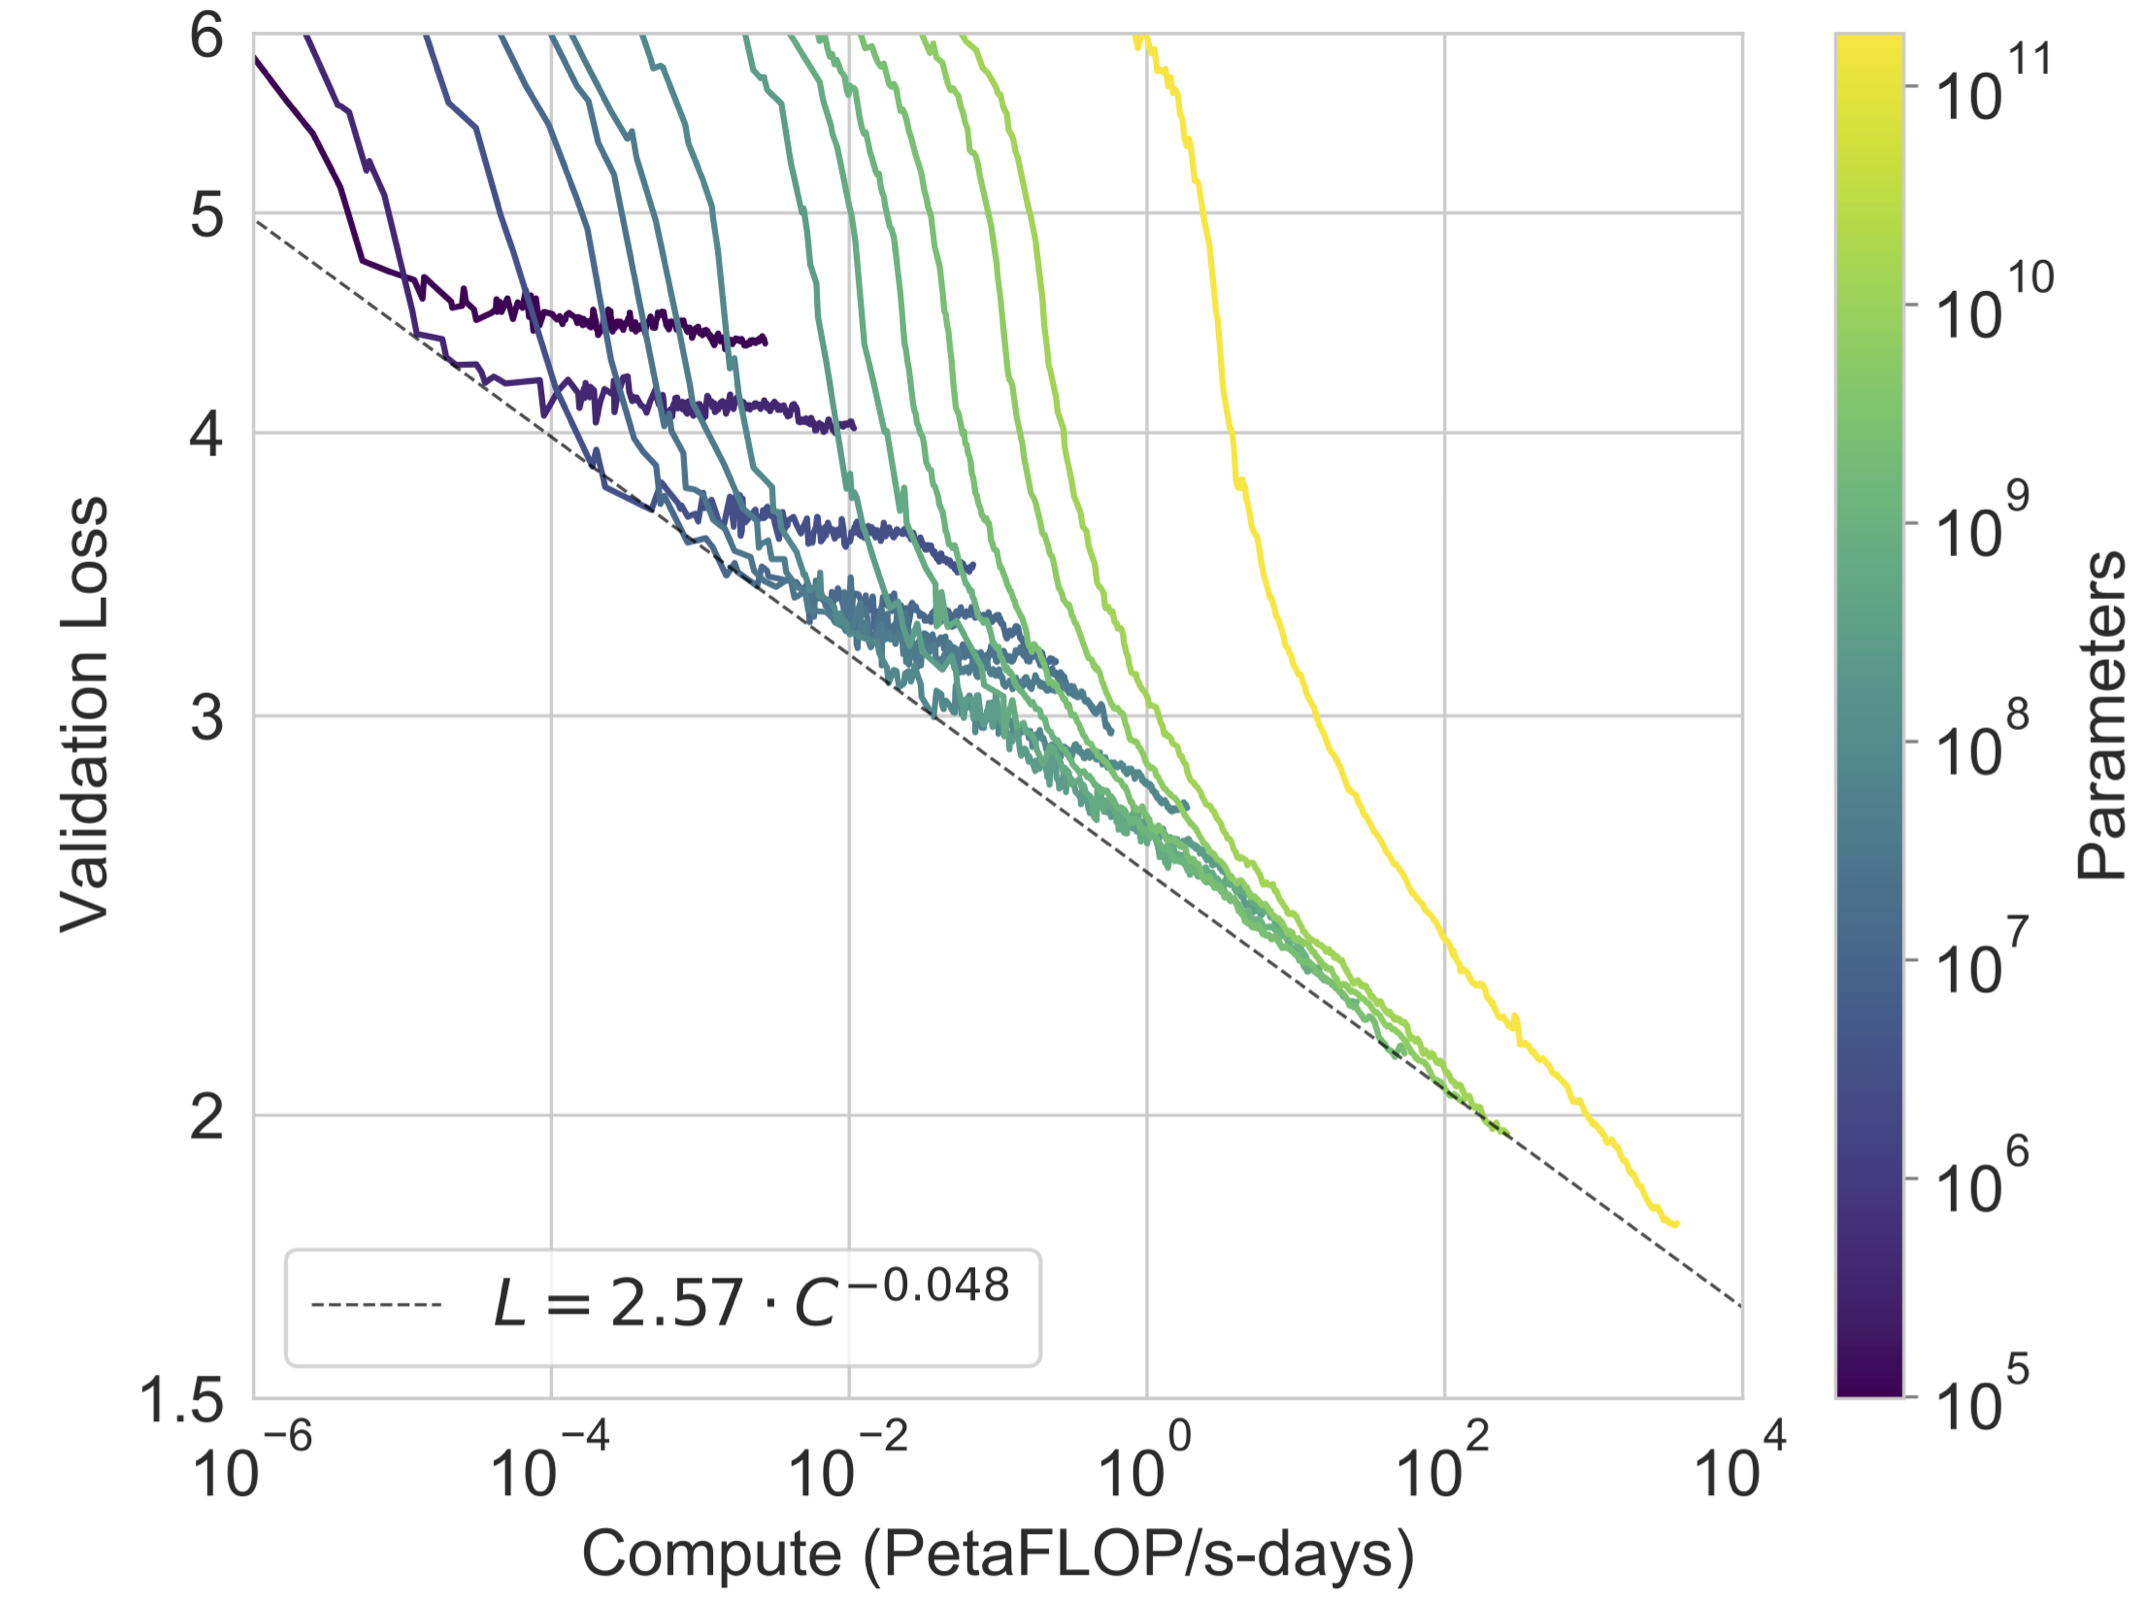
\includegraphics[width=6.5cm]{figure/losscompute.png}
\end{figure}

For a \textbf{fixed model size}, more training initially reduces loss strongly,
but improvements become smaller. Likewise, \textbf{increasing model size} without enough training data
eventually gives diminishing returns.

\begin{center}
\textbf{Good scaling requires balancing model size and training data.}
\end{center}

\end{vbframe}


% ------------------------------------------------------------------------------

\begin{vbframe}{A Scaling Law for Loss}

Loss can be modeled as a function of both model size and training data:

\[
\boxed{
L(P,D)
=
1.61
+
\frac{406.4}{P^{0.34}}
+
\frac{410.7}{D^{0.28}}
}
\]

where

\begin{itemize}
    \item $P$ is the number of parameters,
    \item $D$ is the number of training tokens,
    \item $L(P,D)$ is cross-entropy loss on new text.
\end{itemize}

Increasing either $P$ or $D$ reduces its contribution to the loss,
but with diminishing returns.

\citebutton{Hoffmann et al., 2022}
{https://arxiv.org/abs/2203.15556}

\end{vbframe}

% ------------------------------------------------------------------------------

\begin{vbframe}{How Should We Spend a Fixed Compute Budget?}

Recall:

\[
C \approx 6PD.
\]

Suppose two training runs have the same compute budget:

\[
\begin{array}{c|cc}
 & P & D \\
\hline
A & 10^9 & 10^9 \\
B & 10^8 & 10^{10}
\end{array}
\]

Both have the same product $PD$.

For this exercise, use the simplified scaling law

\[
L(P,D)
=
2
+
\frac{1000}{P^{1/3}}
+
\frac{1000}{D^{1/4}}.
\]

\begin{center}
\textbf{Which configuration should achieve lower loss?}
\end{center}

\end{vbframe}


% ------------------------------------------------------------------------------

\begin{vbframe}{Compute-Optimal Training}

Given a fixed compute budget $C$, choose model size $P$
and training data $D$ to minimize loss:

\[
\boxed{
\text{minimize } L(P,D)
\quad\text{subject to}\quad
6PD = C
}
\]

\citebutton{Hoffmann et al., 2022}
{https://arxiv.org/abs/2203.15556}

Hoffmann et al.\ estimated the optimal trade-off empirically using
hundreds of training runs with different model sizes and dataset sizes.

Their conclusion:

\begin{center}
\textbf{For a fixed compute budget, models should generally be
smaller and trained on more data than previously assumed.}
\end{center}

\end{vbframe}

% ------------------------------------------------------------------------------

\begin{vbframe}{Chinchilla: Smaller Model, More Data}

\citebutton{Hoffmann et al., 2022}
{https://arxiv.org/abs/2203.15556}

Chinchilla was designed to test the compute-optimal prediction.

\begin{itemize}
    \item \textbf{Chinchilla:} 70B parameters, 1.4T training tokens
    \item About \textbf{4$\times$ fewer parameters} than Gopher
    \item About \textbf{4$\times$ more training tokens}
\end{itemize}

Despite being much smaller, Chinchilla

\begin{itemize}
    \item outperformed Gopher,
    \item required less memory for inference,
    \item had lower inference cost.
\end{itemize}

\begin{center}
\textbf{Bigger is not always better: training longer can be a better use of compute.}
\end{center}

\end{vbframe}

% ------------------------------------------------------------------------------

\begin{vbframe}{Were Previous LLMs Too Large?}

\begin{figure}
    \centering
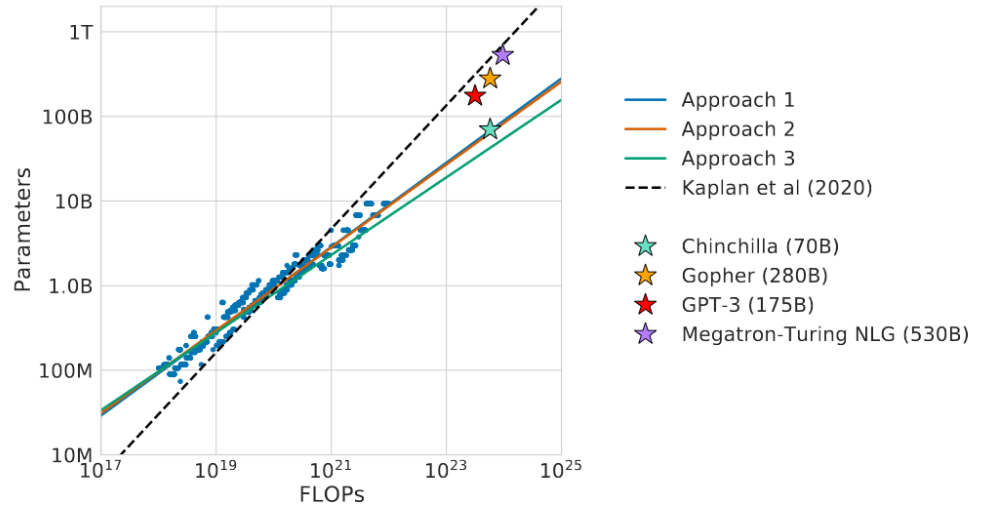
\includegraphics[width=8cm]{./figure/chinchilla.png}
\end{figure}

The Chinchilla scaling law predicted that, for a given compute budget,
many earlier LLMs used \citebutton{Hoffmann et al., 2022}
{https://arxiv.org/abs/2203.15556}

\begin{itemize}
    \item too many parameters,
    \item too few training tokens.
\end{itemize}

\begin{center}
\textbf{Scaling laws shifted compute from model size to data.}
\end{center}
\end{vbframe}

% ------------------------------------------------------------------------------

\begin{vbframe}{Main Takeaway}

Scaling laws make LLM training a \textbf{resource-allocation problem}.

For a fixed compute budget,

\[
C \approx 6PD,
\]

so more parameters mean fewer training tokens, and vice versa.

Empirical scaling laws tell us how to balance both:

\[
\boxed{
\text{choose } P \text{ and } D \text{ jointly, not independently}
}
\]

Chinchilla showed that many earlier LLMs were
\textbf{too large and undertrained} for their compute budget.

A smaller, better-trained model can also reduce
\textbf{inference memory and cost}.

\end{vbframe}

% ------------------------------------------------------------------------------

\begin{vbframe}{Do New Abilities Emerge with Scale?}

Some downstream abilities appear only above a certain model scale.

\begin{itemize}
    \item Small models perform near chance on a task.
    \item Larger models suddenly achieve substantial performance.
    \item This has been called an \textbf{emergent ability}.
\end{itemize}

\begin{figure}
    \centering
    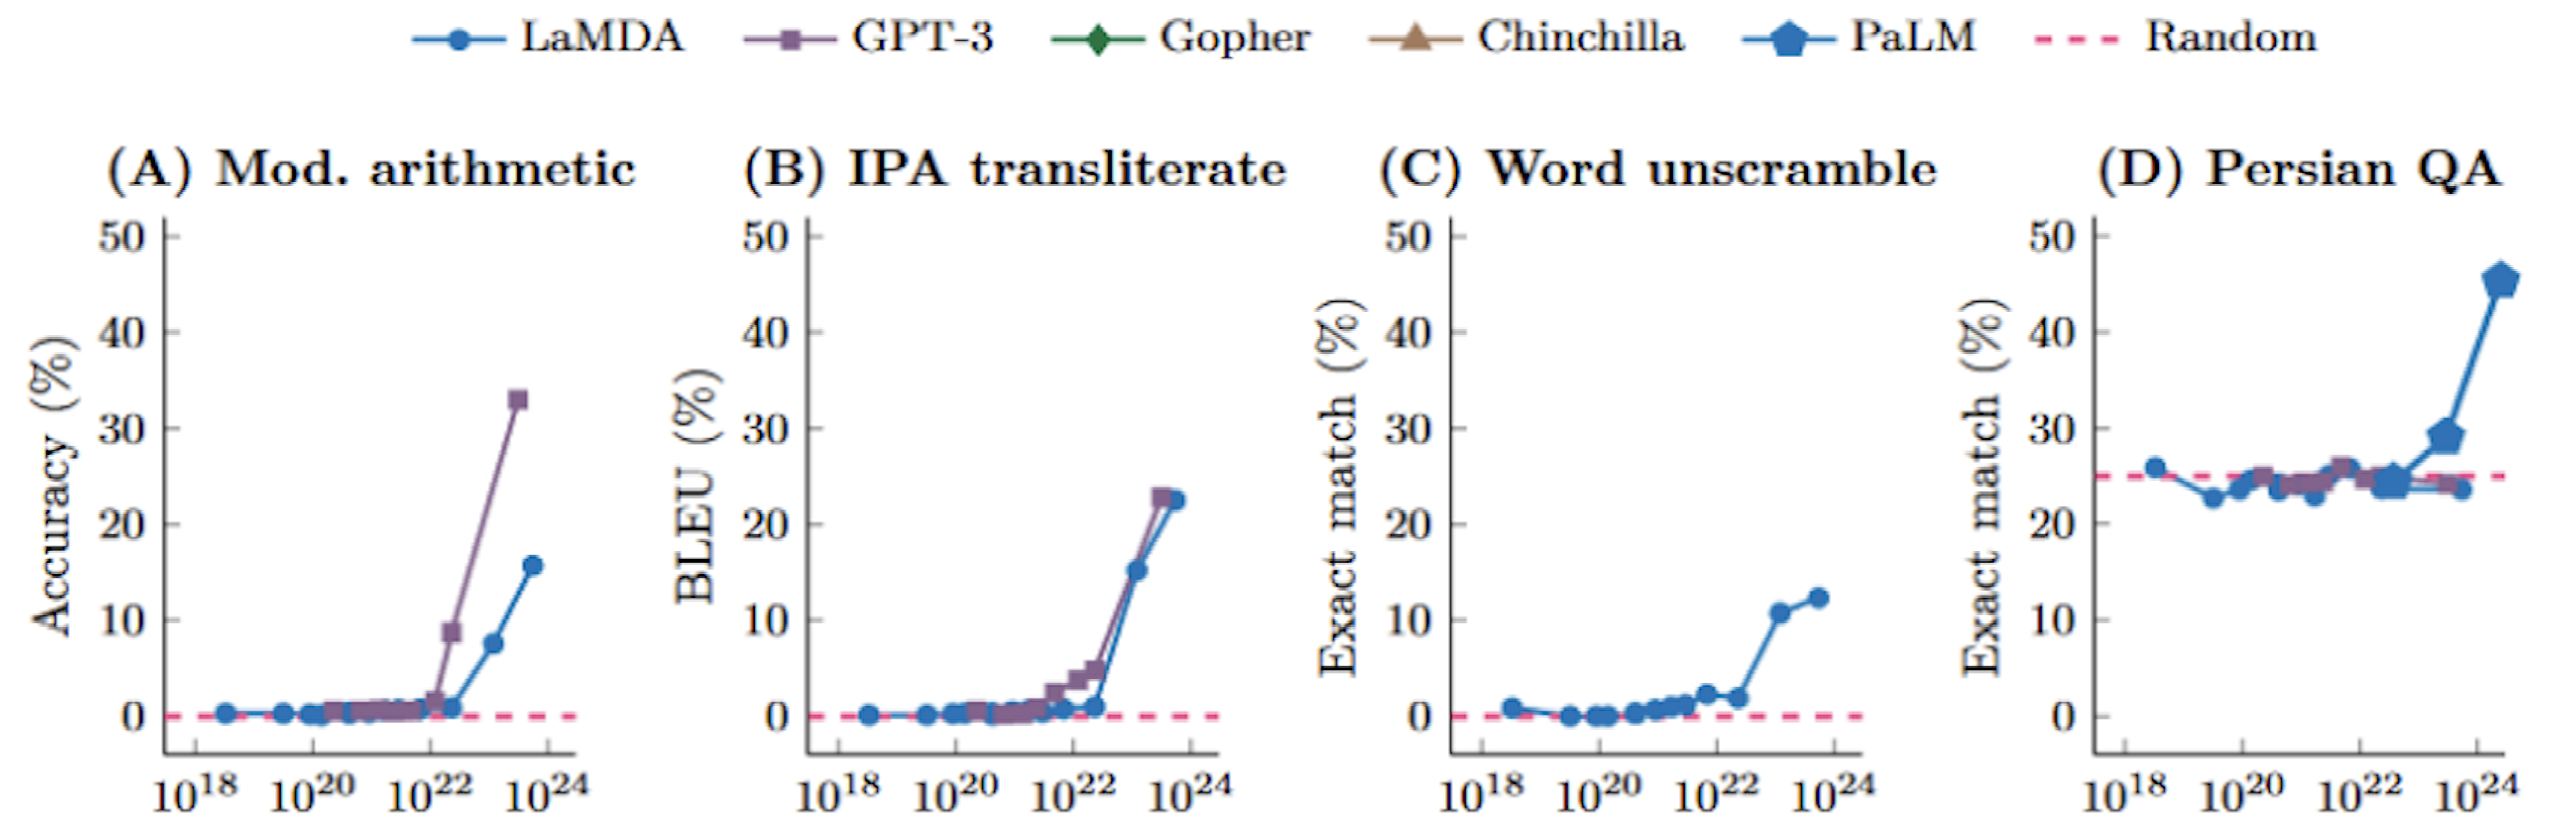
\includegraphics[width=0.85\textwidth]{figure/emergent_abilities2.png}
\end{figure}

\citebutton{Wei et al., 2022: Emergent Abilities of Large Language Models}
{https://arxiv.org/abs/2206.07682}

\end{vbframe}

% ------------------------------------------------------------------------------

\begin{vbframe}{Is Emergence an Artifact of the Metric?}

\citebutton{Schaeffer et al., 2023}
{https://arxiv.org/abs/2304.15004} argue that apparent emergence can arise from
how performance is measured: \textbf{A sudden benchmark jump does not imply
a sudden change in the underlying model.}
\begin{itemize}
    \item Underlying model predictions may improve smoothly with scale.
    \item Discontinuous metrics such as exact match can turn smooth
          improvement into an abrupt jump.
\end{itemize}
\begin{figure}
    \centering
    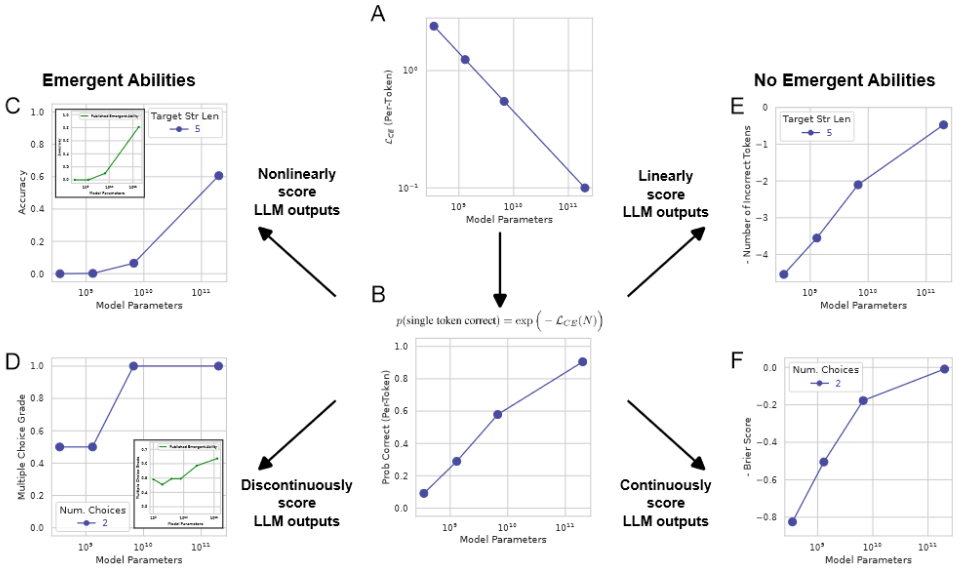
\includegraphics[width=0.67\textwidth]{figure/emergent_experiments.png}
\end{figure}
\end{vbframe}

% ------------------------------------------------------------------------------

\begin{vbframe}{Pretraining Data Are Mixtures}

The number of tokens $D$ does not describe the
\textbf{kind of data}.

\textbf{Example: Dolma} combines several sources

\begin{figure}
    \centering
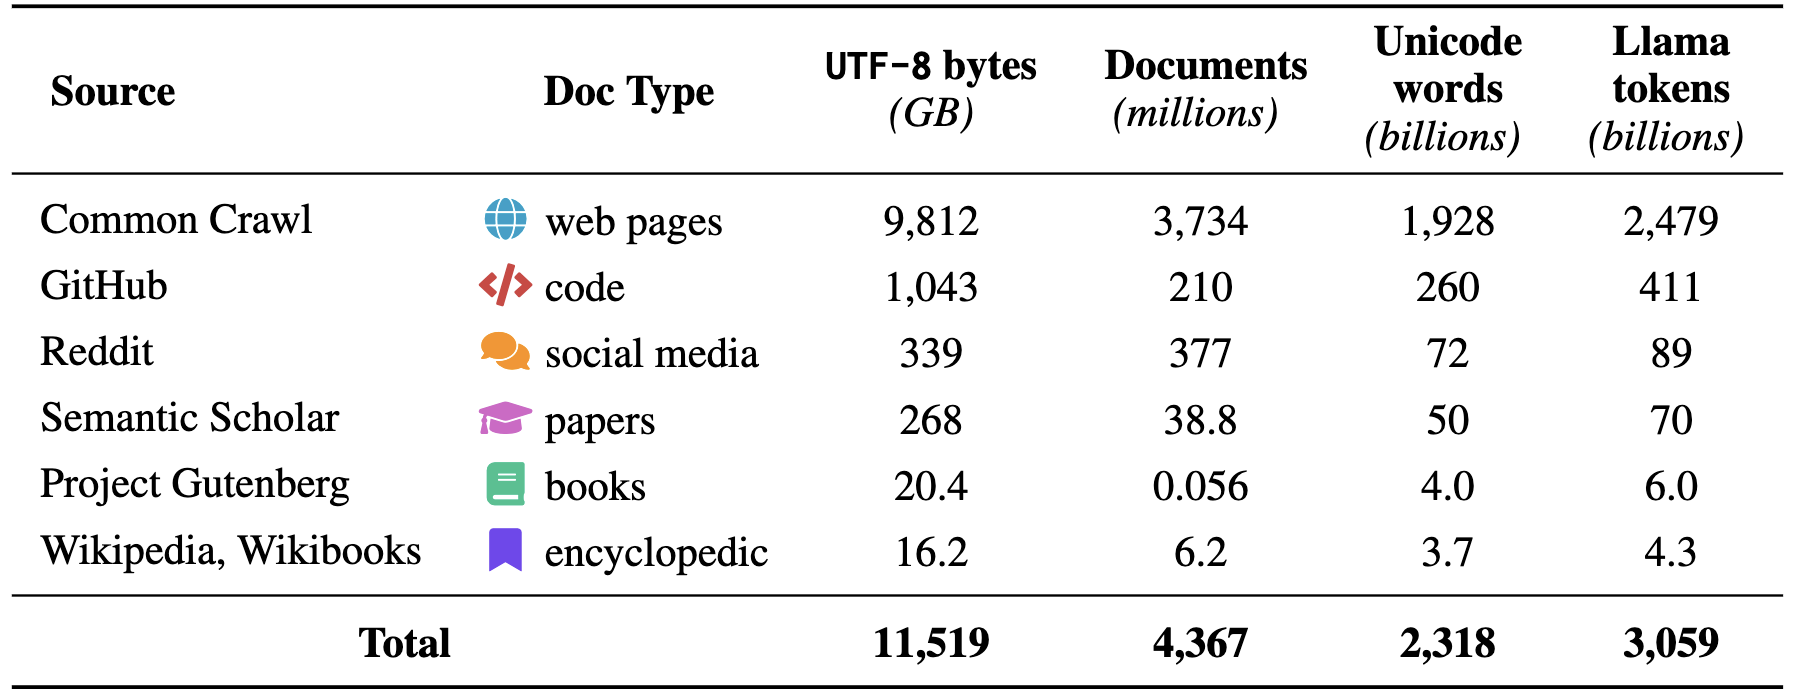
\includegraphics[width=\textwidth]{./figure/dolma.png}
\end{figure}

\citebutton{Soldaini et al., 2024: Dolma}
{https://arxiv.org/abs/2402.00159}

\textbf{The composition of $D$ is itself a design choice.}


\end{vbframe}


% ------------------------------------------------------------------------------
\begin{vbframe}{Which Data Should We Keep?}

\begin{columns}[T]

\begin{column}{0.46\textwidth}

\textbf{Example: FineWeb}


\begin{itemize}
    \item FineWeb contains about \textbf{15T filtered web tokens}.
    \item FineWeb-Edu keeps about \textbf{1.3T tokens} with high predicted
          educational value (``useful for teaching'', judged by an
          LLM-derived classifier).
    \item Models trained on FineWeb-Edu perform better on several
          knowledge and reasoning benchmarks.
\end{itemize}

\end{column}

\begin{column}{0.52\textwidth}

\begin{figure}
    \centering
    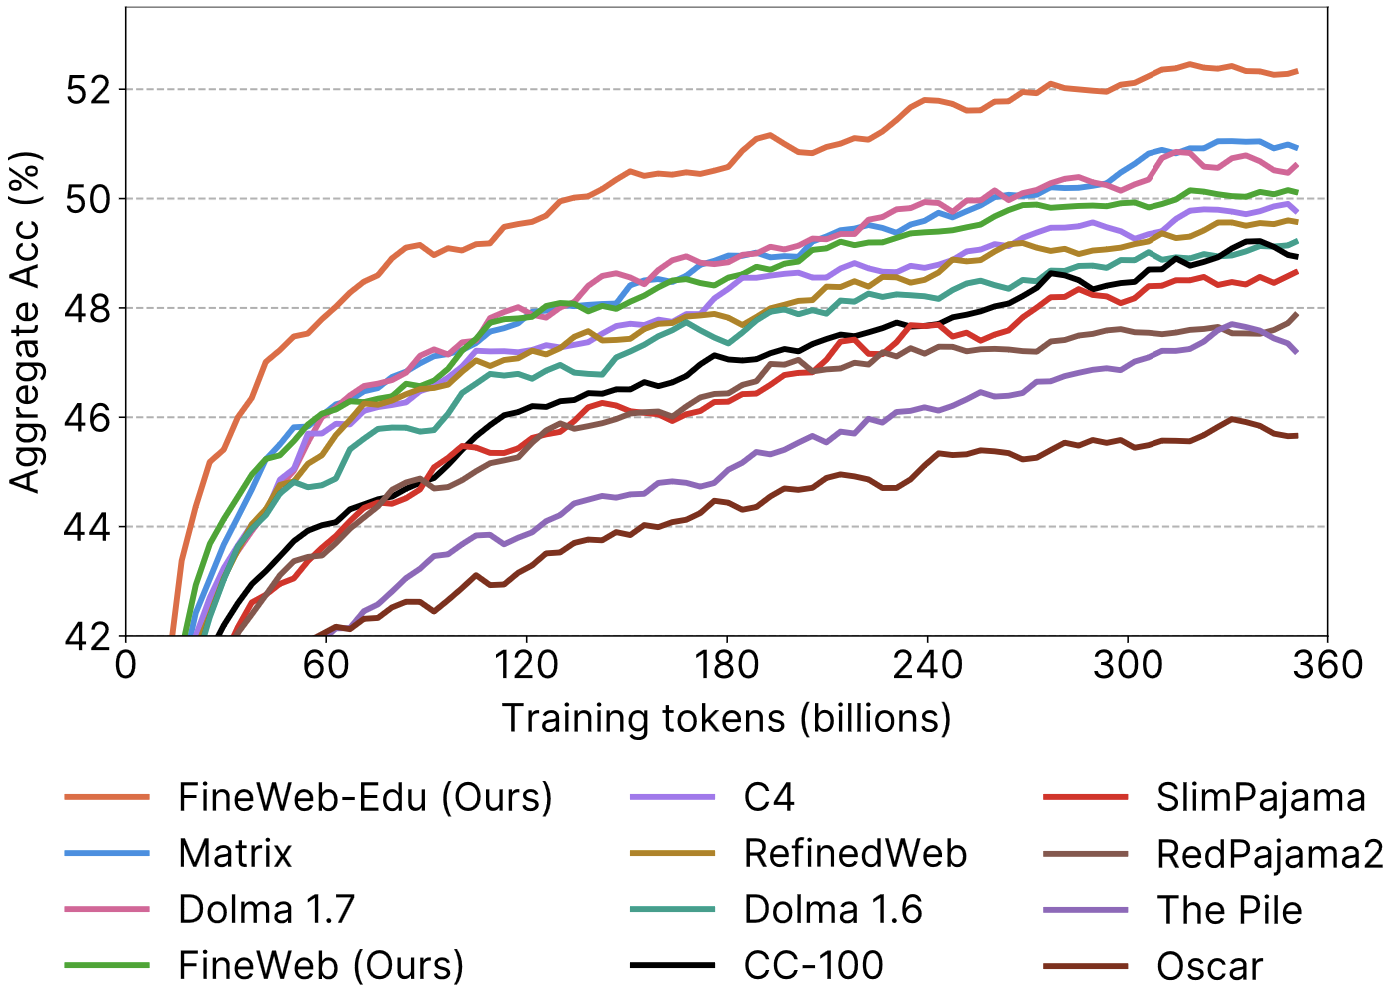
\includegraphics[width=\textwidth]{./figure/fineweb.png}
    \citebutton{Penedo et al., 2024: FineWeb}
{https://arxiv.org/abs/2406.17557}
\end{figure}

\end{column}

\end{columns}

\end{vbframe}


% ------------------------------------------------------------------------------

\begin{vbframe}{What If We Run Out of New Data?}

\begin{columns}[T]

\begin{column}{0.46\textwidth}
If high-quality unique data are limited, one option is to
\textbf{repeat existing data}.

Muennighoff et al.\ find that

\begin{itemize}
    \item a few repetitions almost as useful as fresh unique data,
    \item but additional repetitions increasingly less useful.
\end{itemize}

\end{column}

\begin{column}{0.52\textwidth}

\begin{figure}
    \centering
    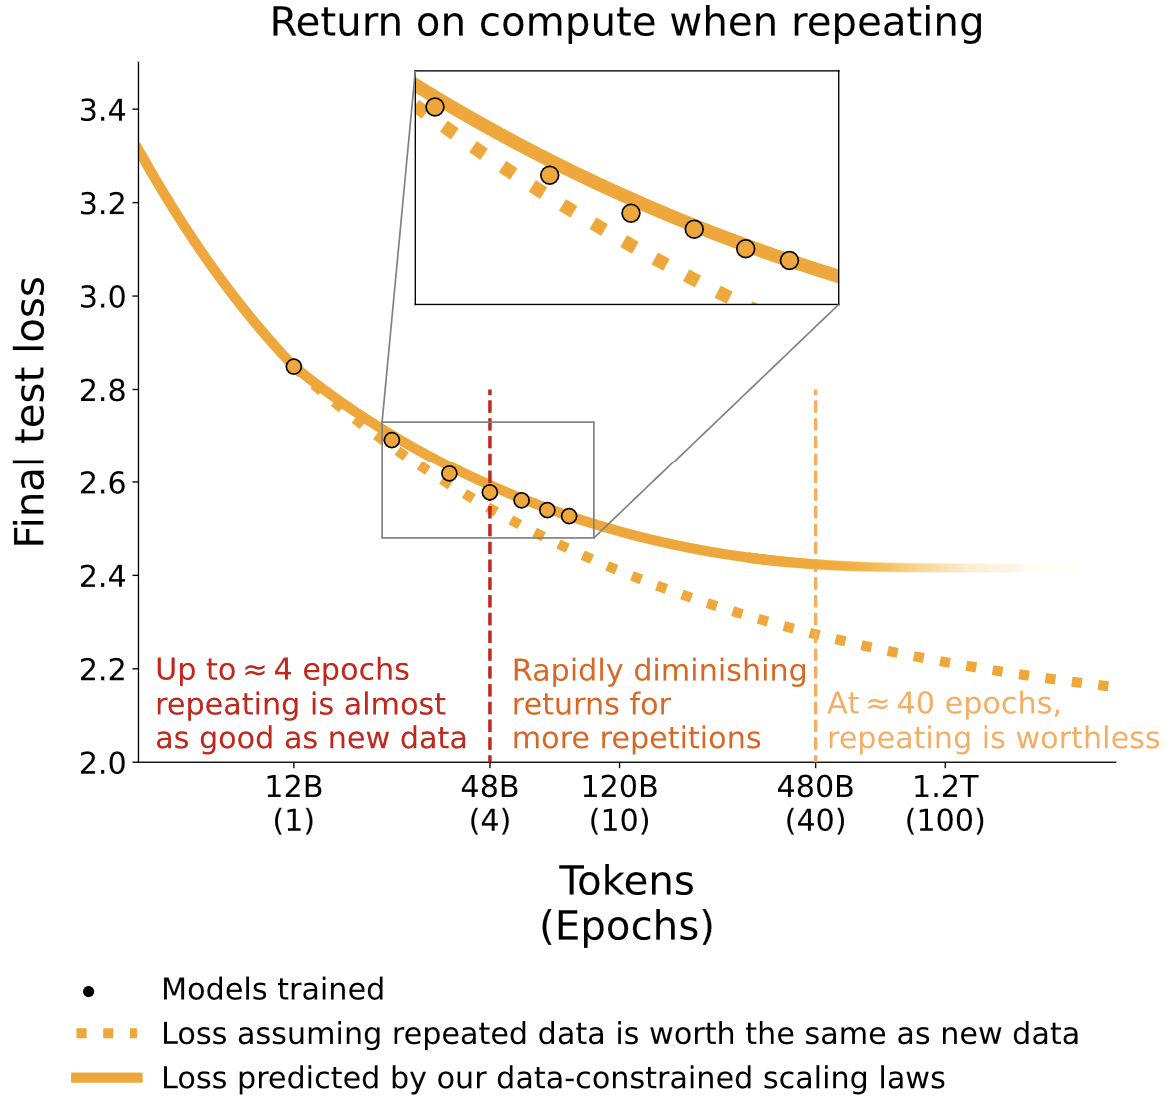
\includegraphics[width=\textwidth]{./figure/muennighoff.png}
\citebutton{Muennighoff et al., 2023}
{https://arxiv.org/abs/2305.16264}
\end{figure}
\end{column}

\end{columns}

\end{vbframe}




% ------------------------------------------------------------------------------
\begin{vbframe}{OLMo 2: Details Make Scaling Work}
Scaling laws say how to allocate compute. The open-source OLMo 2 LLM shows what is needed
so the training run actually remains \textbf{stable}. \citebutton{OLMo Team, 2025: 2 OLMo 2 Furious}
{https\://arxiv.org/abs/2501.00656}


\footnotesize{
\begin{center}
\begin{tabular}{p{0.28\textwidth}p{0.62\textwidth}}
\textbf{Choice} & \textbf{OLMo 2 takeaway} \\
\hline
Repeated text & Filter/mask long repeated $n$-grams; reduces gradient spikes. \\
Initialization & Use $\mathcal{N}(0,0.02)$ for all parameters; fewer spikes and better activation/gradient scaling. \\
Norm placement & RMSNorm on attention/MLP outputs, not inputs. \\
Attention logits & QK-norm prevents very large attention logits. \\
Logit scale & Add z-loss to keep output logits from growing too large. \\
Optimizer details & Lower AdamW $\epsilon$; do not apply weight decay to embeddings. \\
\end{tabular}
\end{center}
}

\end{vbframe}



% ------------------------------------------------------------------------------

\begin{vbframe}{OLMo 2: Short Mid-Training, Large Gains}

After long general pretraining, OLMo 2 performs a much shorter
\textbf{targeted mid-training stage} on filtered higher-quality data.

\vspace{0.15cm}

\begin{center}
\begin{tabular}{lccc}
\textbf{Model} & \textbf{Training tokens} & \textbf{Avg.}\\% & \textbf{GSM8K} \\
\hline
7B
& 4T \textbf{$+$ 150B$^\ast$}
& 53.0 $\rightarrow$ \textbf{62.9}\\%& 24.1 $\rightarrow$ \textbf{67.5} \\

13B
& 5T \textbf{$+$ 600B$^\ast$}
& 58.9 $\rightarrow$ \textbf{68.3}\\%& 37.3 $\rightarrow$ \textbf{75.1} \\

32B
& 6T \textbf{$+$ 600B$^\ast$}
& 66.3 $\rightarrow$ \textbf{73.3}\\%& 56.2 $\rightarrow$ \textbf{78.8} \\
\end{tabular}
\end{center}

\vspace{0.15cm}

{\scriptsize
$^\ast$\textbf{Total mid-training compute across several continuations:}
7B: $3\times 50$B;
13B/32B: $3\times 100$B $+$ 300B.
All runs start from the same pretrained checkpoint and their final
checkpoints are \textbf{averaged (model soup)}.
}

\vspace{0.25cm}

\begin{itemize}

    \item Mid-training switches to the curated
          \textbf{Dolmino-Mix-1124} mixture and anneals the learning rate.

    \item Despite requiring far fewer tokens than general pretraining,
          it yields \textbf{large improvements}.

\end{itemize}

\citebutton{OLMo Team, 2025: 2 OLMo 2 Furious}
{https\://arxiv.org/abs/2501.00656}

\end{vbframe}

% ------------------------------------------------------------------------------

\begin{vbframe}{Scaling Has a Financial Cost}

Estimates for training frontier models, based on cloud-compute rental prices (not total development costs):

\begin{itemize}
    \item Estimated training compute cost:
          \textbf{GPT-3: \$4M}, \textbf{GPT-4: \$79M},
          \textbf{Llama 3.1-405B: \$170M}.
    \item Experiments, tuning, and failed runs add further cost.
\end{itemize}


\begin{figure}
    \centering
    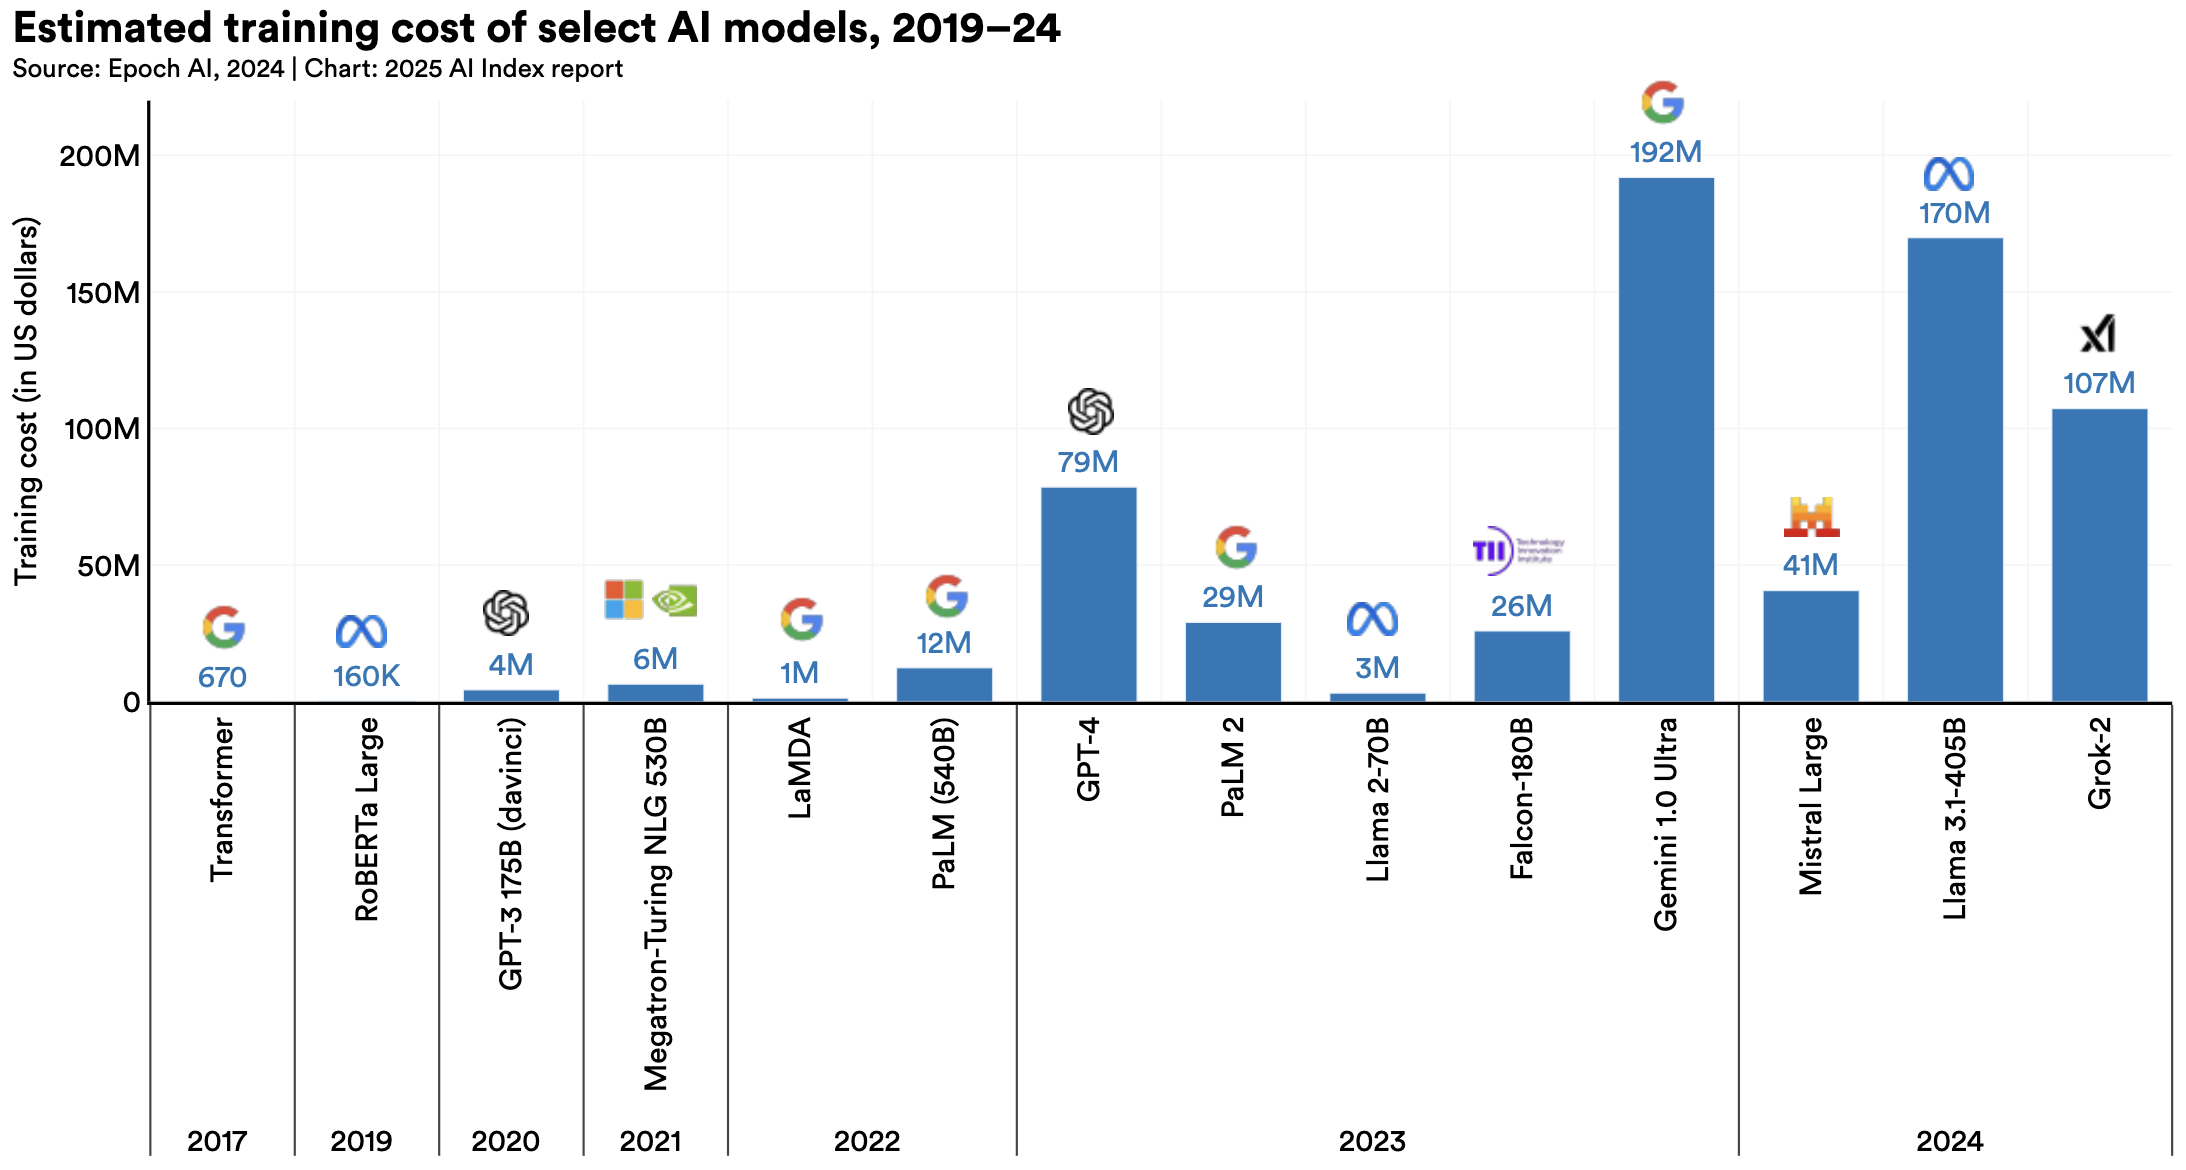
\includegraphics[width=0.77\textwidth]{./figure/training_costs.png}
\citebutton{Stanford AI Index, 2025}
{https://hai.stanford.edu/assets/files/hai_ai_index_report_2025.pdf}
\end{figure}


\end{vbframe}

\begin{vbframe}{Environmental Costs of Training}

\begin{itemize}
    \item Estimated training emissions:
          \textbf{GPT-3: 588 t}, \textbf{GPT-4: 5,184 t},
          \textbf{Llama 3.1-405B: 8,930 t CO$_2$e}.
    \item Emissions depend on hardware efficiency, datacenter efficiency,
          and the carbon intensity of electricity.
    \item Patterson et al.\ observed about \textbf{5--10$\times$}
          differences across locations. \citebutton{Patterson et al., 2021}
{https://arxiv.org/abs/2104.10350}
\end{itemize}

\begin{figure}
    \centering
    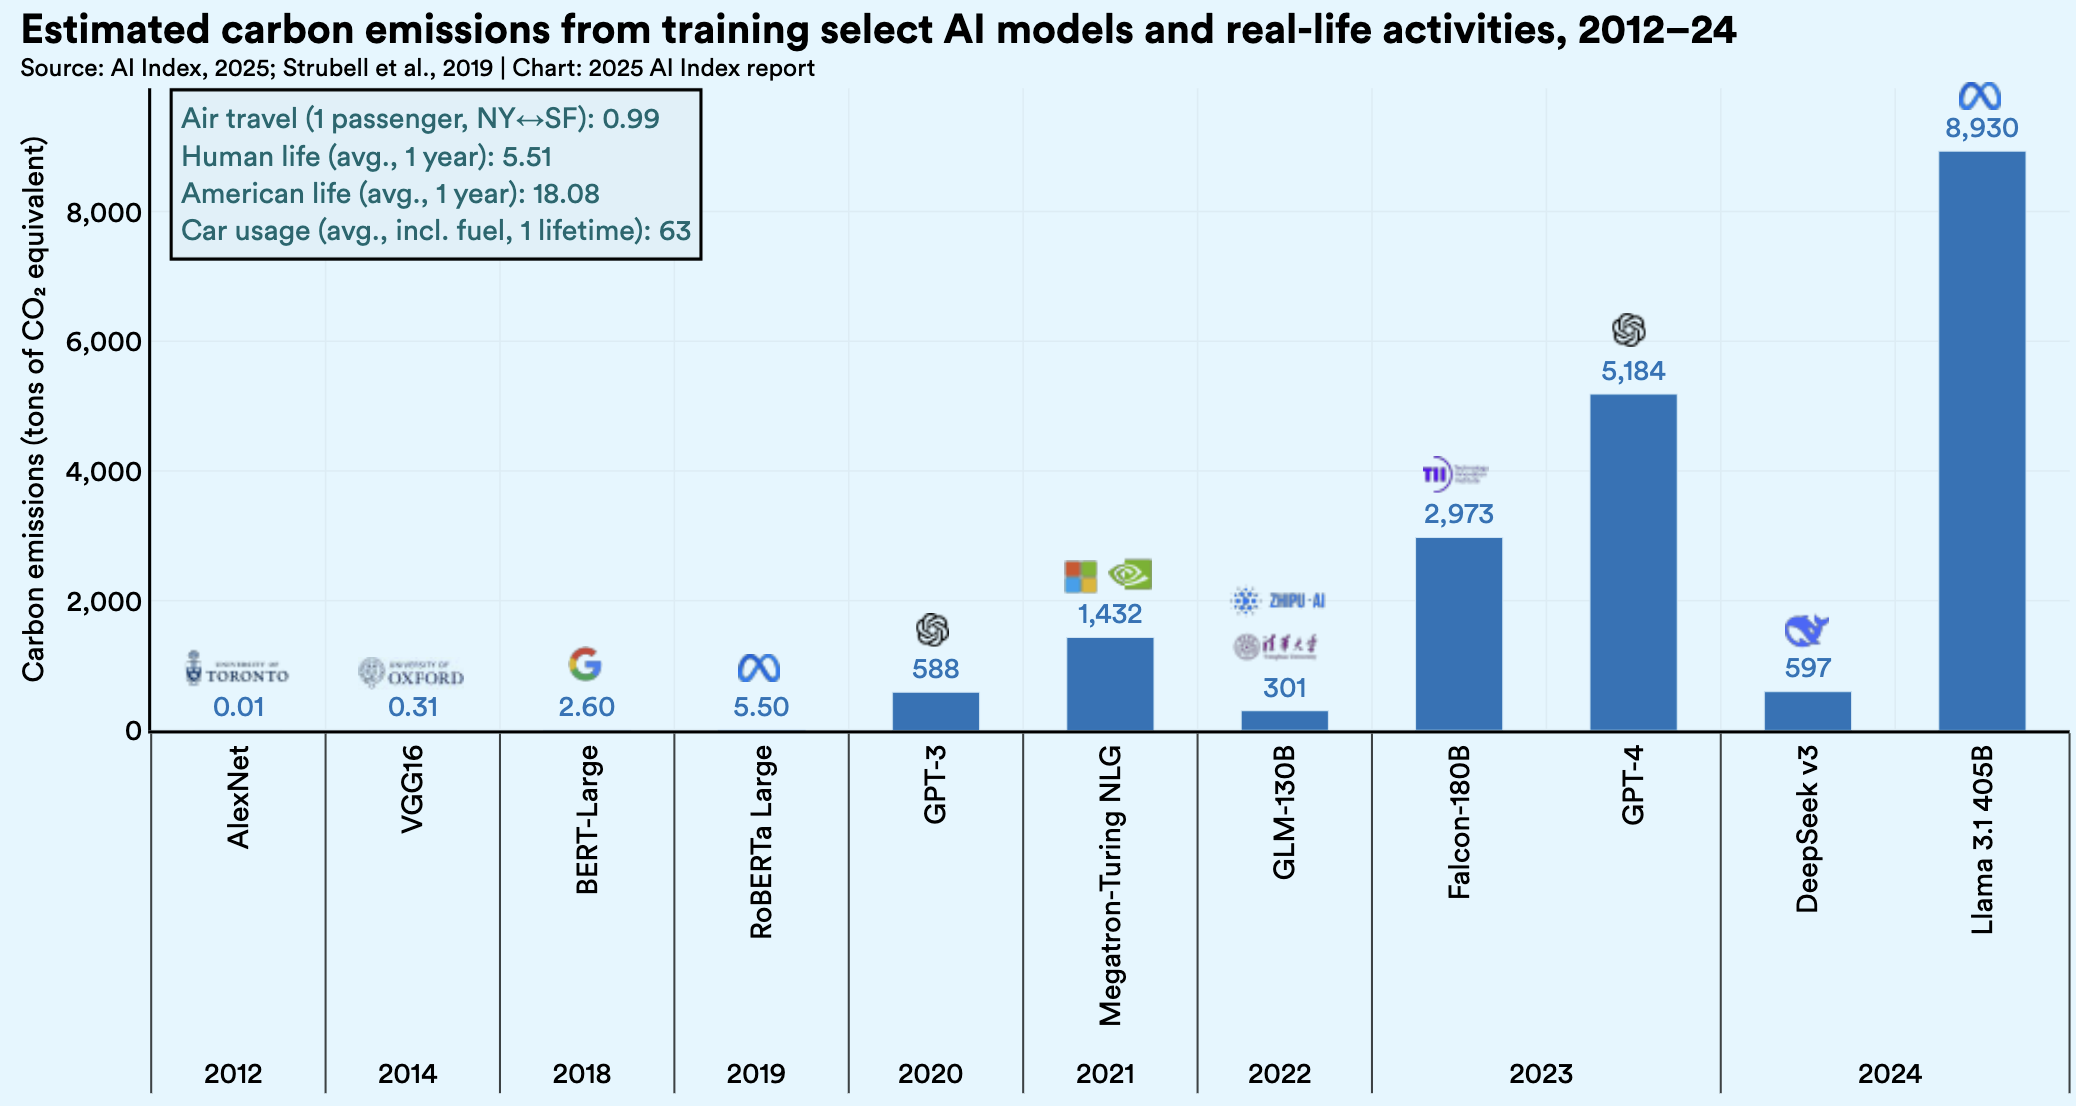
\includegraphics[width=0.77\textwidth]{./figure/co2_emissions.png}
\citebutton{Stanford AI Index, 2025}
{https://hai.stanford.edu/assets/files/hai_ai_index_report_2025.pdf}
\end{figure}


\end{vbframe}




\endlecture
\end{document}
